\section{Felder}
\subsection{Zusammenhänge}
Materialgleichungen
\begin{align*}
    \Aboxed{\vec{J}  = \kappa\vec{E}} &
    \Aboxed{\vec{B}  = \mu\vec{H}}    &
    \Aboxed{\vec{D}  = \varepsilon\vec{E}}\\
    \Aboxed{ rot \vec{H} = \vec{J} = \sigma \cdot \vec{E}} &
\end{align*}

\begin{align*}
    \Aboxed{&\oint{\vec{H} \, d\vec{s}} = \Theta = I = \iint_A \vec{J}  \, d\vec{A} = \frac{d\Phi_e}{dt}} \\
    \Aboxed{&\oint{\vec{E} \, d\vec{s}} = u_{ind} = -\frac{d}{dt}\iint{\vec{B} \, d\vec{A}} = -\frac{d\Phi_m}{dt}} \\
    \Aboxed{&rot{\vec{E}} = -\frac{\partial\vec{B}}{\partial t} = -\mu\cdot\frac{\partial\vec{H}}{\partial t} = -j\omega\mu\vec{H}}
\end{align*}

Feldunterscheidung
\begin{align*}
     & \vec{E}(x,y,z)                               & \widehat= & \quad\text{statisches Feld}  & \\
     & \vec{E}(x,y,z,t)                             & \widehat= & \quad\text{stationäres Feld} & \\
     & \vec{E}(x,y,z,t)\cdot cos(\omega t -\beta z) & \widehat= & \quad\text{Welle}            &
\end{align*}

\subsection{Elektrostatik}
\textbullet wirbelfreies Feld $\rightarrow$ Elektrische Ladungen sind Quellen des
Feldes
\begin{align*}
    \Aboxed{\opdiv \vec{D} & = \nabla \cdot \vec{D}  = \rho}\\
    \Aboxed{\oprot \vec{E} & = \nabla \times \vec{E} = 0} \quad \Aboxed{\oprot \opgrad E & = 0}\\
    \Aboxed{\vec{E} & = - \opgrad \varphi} \\
    Q &= \iiint_V \rho \, dV \\
    U_{ab} &= \int_{a}^{b} E \, ds
\end{align*}

\subsubsection{Potential Gleichung}
\[
    \opdiv \opgrad \varphi = - \dfrac{\rho}{\varepsilon}
\]

\textbf{$\qquad \Rightarrow$ Poisson-Gleichung}\\
mit $\rho = 0$ $\rightarrow$ \textbf{Laplace-Gleichung}
\begin{align*}
    \Delta \varphi + \underbrace{ \dfrac{\opgrad \varepsilon \cdot \opgrad \varphi}{\varepsilon}}_{= 0\texttt{, wenn homogen}}
     & = - \dfrac{\rho (x, y, z)}{\varepsilon} \\
    \frac{d^2 \varphi}{d x^2} + \frac{d^2 \varphi}{d y^2} + \frac{d^2 \varphi}{d z^2}
     & = - \dfrac{\rho (x, y, z)}{\varepsilon}
\end{align*}

\subsubsection{Green'sche Funktionen}
\textbf{Potential einer Punktladung}
\[ \varphi (r) = \dfrac{Q}{4 \pi \varepsilon_0 \cdot r} \qquad\left[V\right]\] 

\textbf{Potentialfeld einer Ladungsverteilung}

mit $\varphi(\infty)=0$
\[
    \varphi(x, y, z)=\frac{1}{4 \pi \varepsilon} \iiint_{V^{\prime}}
    \frac{\rho\left(x^{\prime}, y^{\prime},
        z^{\prime}\right)}{\left|\vec{r}-\vec{r}^{\,\prime}\right|} \mathrm{d}
    V^{\prime}
\]

mit der Green'schen Funktion $G\left(\vec{r}, \vec{r}^{\,\prime}\right)=\frac{1}{4 \pi \varepsilon\left|\vec{r}-\vec{r}^{\,\prime}\right|}$
\[\varphi(x, y, z)=\iiint_{V^{\prime}} G\left(\vec{r}^{\,\prime} \vec{r}^{\,\prime}\right) \rho\left(\vec{r}^{\,\prime}\right) \mathrm{d} V^{\prime}\]


\textbf{E-Feld einer Punktladung}
\[ \vec{E}(r) = \dfrac{Q}{4 \pi \varepsilon_0 \cdot r^2}\cdot\vec{e}_r \qquad\left[\frac{V}{m}\right]\] 

\textbf{D-Feld einer Punktladung}
\[ \vec{D}(r) = \dfrac{Q}{4 \pi \cdot r^2}\cdot\vec{e}_r \qquad\left[\frac{As}{m^3}\right]\]

\subsubsection{Elektrischer Dipol}

\begin{align*}
    \Aboxed{\vec{p} = Q\cdot\vec{d}}
\end{align*}

\makebox[0pt][l]{
    \begin{minipage}[b]{0.5\columnwidth}
        \input{Figures/Felder_Elektrischer_Dipol_1.tex}
    \end{minipage}
    \begin{minipage}[b]{0.5\columnwidth}
        \input{Figures/Felder_Elektrischer_Dipol_2.tex}
    \end{minipage}
}

\makebox[0pt][l]{
    \begin{minipage}[]{0.5\columnwidth}
        \begin{align*}
            \varphi & = \frac{Q}{4\pi\varepsilon_0}\left(\frac{1}{r_1}-\frac{1}{r_2}\right)                                        \\
                    & = \frac{Q}{4\pi\varepsilon_0}\cdot\frac{r_2-r_1}{r^2}                                                        \\
            \vec{E} & = -\nabla\varphi                                                                                             \\
                    & = \frac{1}{4\pi\varepsilon_0}\cdot\left(\frac{3(\vec{p}\cdot\vec{r})\vec{r}}{r^5}-\frac{\vec{p}}{r^3}\right)
        \end{align*}
    \end{minipage}

    \begin{minipage}[]{0.5\columnwidth}
        \begin{align*}
            \varphi & \approx\frac{Qd\cos\theta}{4\pi\varepsilon_0r^2}                  \\
                    & = \frac{1}{4\pi\varepsilon_0}\cdot\frac{\vec{p}\cdot\vec{r}}{r^3}
        \end{align*}
    \end{minipage}
}


\subsection{Magnetostatik}
\textbullet Wirbelfeld, quellenfrei und hat immer \underline{geschlossene} Feldlinien.\\
\textbullet Nach $rot \vec{H} = j$ $\rightarrow$ nur wirbelfrei wenn $j = 0$\\
\textbullet Damit Skalarpotential $ \varphi_m$ existiert muss H wirbelfrei\\
\textbullet keine magnetischen Monopole $grad \vec{B} = 0$\\
\textbullet Vektorpotential $ \vec{A}$ = Maß für $\Phi_{magn} $ durch Fläche A
\begin{align*}
    \Aboxed{\oprot \vec{H} = \nabla \times \vec{H} & = \vec{J} }          & \vec{B} & = \mu \vec{H}           \\
    \vec{H}                                        & = - \nabla \varphi_m &                                   \\
    \Aboxed{\opdiv \vec{B} = \nabla \cdot \vec{B}  & = 0 }                &         & = \opdiv \oprot \vec{B}
\end{align*}
\textbf{Coulomb-Eichung}
\begin{align*}
    \Delta \vec{A} & = - \mu \vec{J}  \\
    \vec{B}        & = \oprot \vec{A}
\end{align*}

\subsubsection{Vektorpotential in Abhängigkeit von der Stromdichte}
\[
    \vec{A}(x, y, z)=\frac{\mu}{4 \pi} \iiint_{V^{\prime}} \frac{\vec{J}\left(x^{\prime}, y^{\prime}, z^{\prime}\right)}{\left|\vec{r}-\vec{r}^{\,\prime}\right|} d V^{\prime}
\]

\subsubsection{Biot-Savart-Gesetz}
\[
    \vec{H}=\frac{I}{4 \pi} \oint_{C^{\prime}} \opgrad \frac{1}{\left|\vec{r}-\vec{r}^{\,\prime}\right|} \times \mathrm{d} \vec{s}^{\,\prime}
\]

mit $\opgrad \frac{1}{\left|\vec{r}-\vec{r}^{\,\prime}\right|}=-\frac{\vec{r}-\vec{r}^{\,\prime}}{\left|\vec{r}-\vec{r}^{\,\prime}\right|^{3}}$

\[
    \vec{H}=\frac{I}{4 \pi} \oint_{C^{\prime}} \frac{\mathrm{d} \vec{s}^{\,\prime} \times\left(\vec{r}-\vec{r}^{\,\prime}\right)}{\left|\vec{r}-\vec{r}^{\,\prime}\right|^{3}}
\]

{\footnotesize$\vec{r}:$ Aufpunkt $\quad \vec{r}^{\,\prime}:$ Quellpunkt}
\[
    H = \frac{I}{2 \pi A} ( \cos(\alpha_1) - \cos(\alpha_2))
\]
{\footnotesize$\alpha_1, \alpha_2$ gleicher Ursprung !, A kürzester Abstand}

\subsubsection{Magnetischer Dipol}
\input{Figures/Felder_Magnetischer_Dipol_1.tex}

\begin{align*}
    I\textnormal{ entlang Leiter }                                                                                                                                        \\
    A(r)                            & = \frac{\mu_0 \cdot I}{4 \pi} \int \frac{d \vec{s}}{| \vec{r} - \vec{s}|} = \frac{ \mu_0}{4 \pi} \frac{\vec{m} \times \vec{r}}{r^3} \\
    \vec{B} = \nabla \times \vec{A} & = \frac{\mu_0}{4 \pi} \left(\frac{3(\vec{m} \cdot \vec{r})\vec{r}}{r^5} - \frac{\vec{m}}{r^3}\right)
\end{align*}

\newpage
\subsection{Skineffekt}

\begin{center}
    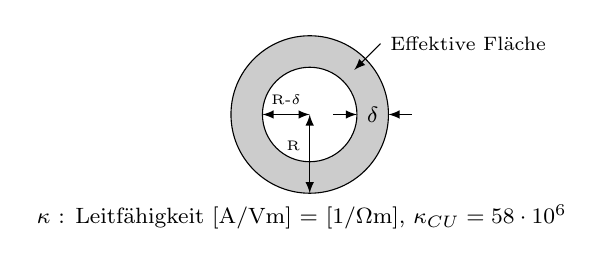
\begin{tikzpicture}
        %Kreise
        \draw[-,fill=black!20] (0,0) circle (1);              %äußerer Kreis
        \draw[-,fill=white] (0,0) circle (0.6);               %innerer Kreis

        %Pfeile
        \draw[latex-latex] (-0.6,0) -- (0,0) node[midway, above]{\tiny{R-$\delta$}};
        \draw[latex-latex] (0,-1) -- (0,0) node at (0,-0.4) [left]{\tiny R};

        \node at (0.8,0)[]{\footnotesize$\delta$};
        \draw[-latex] (0.3,0) -- (0.6,0);
        \draw[latex-] (1,0) -- (1.3,0);

        \draw[latex-] (0.566,0.566) -- (.9,.9) node[above, right]{\scriptsize{Effektive Fläche}};

        %Legende
        \node at (-0.1,-1.3)[]{\footnotesize{$\kappa$ : Leitfähigkeit [A/Vm] = [1/$\Omega$m], $\kappa_{CU} = 58 \cdot 10^6$}};
    \end{tikzpicture}
\end{center}


\begin{description}
    \item Äquivalente Leiterschichtdicke (Amp: $A \cdot \frac{1}{e}$):
          \[
              \delta = \frac{1}{\sqrt{\pi\mu\kappa f}} = \sqrt{\frac{2}{\omega\mu\kappa}} \qquad \left[ m \right] \\
          \]

    \item Widerstand/Oberflächenwiderstand:
        \begin{flalign*}
            R_{AC} & = \frac{l}{\kappa \cdot A_{\texttt{eff}}} \\
            R_{DC} & =\dfrac{l}{\kappa \pi R^{2}}  = \frac{l}{\kappa A}          \\
            R_{OF} & = \dfrac{1}{\kappa \delta}
        \end{flalign*}

    \item \textbf{Feldstärke} verglichen mit der Oberfläche:
    \item analog für $E$-Feld
        \[
            H\left( x,t\right) = H_{0}\cdot e^{^{-x}/_\delta}\cdot \cos \left( \omega t-\dfrac{x}{\delta}\right)\\
        \]  
    \item
        \[
            \hat{H} = \sqrt{\frac{\kappa}{\omega \mu}} \cdot \hat{E}
        \]

    \item \textbf{Leistung} verglichen mit der Oberfläche:
        \[
            P\left( x,t\right) = \dfrac{1}{2} \cdot E_{0}\cdot e^{^{-x}/_\delta}\cdot H_{0}\cdot e^{^{-x}/_\delta}
        \]

    \item Amplitude und Phase bezogen auf $\delta$:
    \item mit $F =$ Dämpfungsfaktor
        \begin{align*}
            \text{Amplitude: } x   & = \ln(F) \qquad \left[\delta\right] \\
            \text{Phase: } \varphi & = -\frac{x}{\delta}
        \end{align*}

    \item Effektive Fläche:
        \begin{align*}
            A_{\texttt{eff}} & = A_{\texttt{ges}} - A_{\kappa} = R^2\pi-(R-\delta)^2\pi \\
                            & = 2\cdot \pi \delta \left( R-\dfrac{\delta }{2}\right)
        \end{align*}
\end{description}

Wenn die Länge nicht gegeben ist oder nach Wieviel \% nimmt der Widerstand bei
einer bestimmten Frequenz, kann dies mit der folgenden Formel berechnet werden:

\begin{description}
    \item Bessel-Funktion:
        \begin{align*}
            \frac{R_{AC}}{R_{DC}} & =
            \begin{dcases}
                1 + \frac{1}{3}x^4              & \text{für} \qquad x < 1 \\
                x + \frac{1}{4} + \frac{3}{64x} & \text{für} \qquad x > 1 \\
            \end{dcases} \\
            \frac{X_{AC}}{R_{DC}} & =
            \begin{dcases}
                x^2\left( 1-\frac{x^4}{6} \right)   & \text{für} \qquad x < 1 \\
                x- \frac{3}{64x} + \frac{3}{128x^2} & \text{für} \qquad x > 1 \\
            \end{dcases}
        \end{align*}
        \[
            \boxed{x=\frac{r_0}{2\delta}} \qquad r_0 \hat{=} \textnormal{ Außendurchmesser}
        \]
\end{description}